\documentclass[11 pt]{amsbook}
\usepackage{../HBSuerDemir}

\begin{document}
\hPage{b2p2/275}

on the paraboloid $ S: z = x^2 + y^2$. There is discontinuity when $P_0 \in S$. The discontinuity may be removable along the curve of intersection of the surfaces $ S: z - x^2 - y^2$, $ T: 2x - y^2 + z = 0$. \par
The properties and Theorems on continuity on continuous functions are valid for function of several variables.
\begin{exmp}[Given the function]

\begin{equation}
\frac{x}{2} + \frac{y}{4} + \frac{z}{5} = 1
\end{equation}
defined on $R_{xy} = (0, 1; 0, 1-x)$
\begin{itemize}
\item[a)] find m and M for z,
\end{itemize}
\begin{itemize}
\item[b)] find points on $R_{xy}$ such that $\mu = \frac{1}{2}$ (m + M)
\end{itemize}
\end{exmp}
\begin{hSolution}

\begin{minipage}{0.6\textwidth}\
a) $ z = (20 - 10x - 5y)/4$ is max when\\

x = 0 and y = 0. Then M = 5.\par

From the figure, min z occurs\\

 either at A or at B:\par


$z(A) = 5/2, z(B) = 15/4 \Rightarrow m=5/2.$\\

b) $\mu = \frac{1}{2} ( \frac{5}{2} + 5) = \frac{15}{4}$ \\

$\Rightarrow \frac{15}{4} = \frac{(20 - 10x - 5y)}{4} \Rightarrow 2x +y = 1$

\begin{equation}
(x, y) \in [BC].
\end{equation}
\end{minipage}
\noindent\begin{minipage}{0.3\textwidth}\flushright
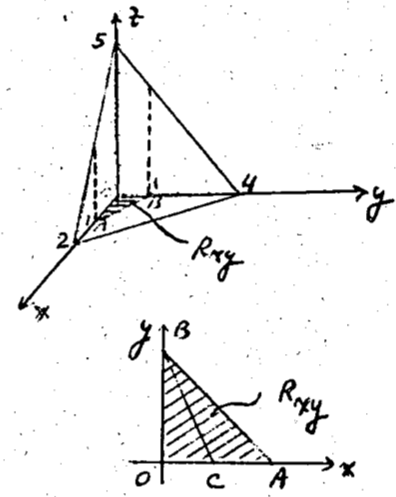
\includegraphics[width=\linewidth]{images/image}
\end{minipage}%

\par 

In complicated cases, solution may involve solution of max min problems of functions of several variables.
\end{hSolution}
\begin{exercise}{Exercise}[4.1]
1. Which ones of the following relations are functions of x and y?
\end{exercise}
\end{document}

